% !TeX program = lualatex
% !TeX encoding = utf8
% !TeX spellcheck = uk_UA

\documentclass[]{beamer}
\usetheme{PlasmaPhysics}
\usepackage{PlasmaPhysics}
\setlength{\abovedisplayskip}{3pt}
\setlength{\belowdisplayskip}{3pt}
\usetikzlibrary{decorations.pathreplacing}
\newtcolorbox{mysidebyside}[1][]{
    notitle, sidebyside, blanker,
    sidebyside align=center seam,
    halign=center,
    lefthand width=.5\textwidth,
    #1
}



\graphicspath{{pictures/}}
\title[Лекції з фізики плазми]{\bfseries\huge Основні характеристики\\ плазми}
\subtitle{\bfseries Лекції з фізики плазми}
\author{Пономаренко С. М.}
\date{}
% https://www.youtube.com/watch?v=zv9Y7YmHyBk
\def\stext#1{\text{
        \makebox[0pt]{
            \tikz[baseline] {\node[text width=50pt, align=center, execute at begin node=\setlength{\baselineskip}{-0.5ex}, blue] {#1};}
        }
}}

\setbeamercovered{transparent=25}

%% --------------------------------------------------------
% Радіус Дебая
\NewDocumentCommand{\rD}{}{
    r_D = \sqrt{\frac{T}{4\pi e^2n}}
}

% Плазмова частота
\NewDocumentCommand{\omegap}{}{%
    \omega_p = \sqrt{\frac{4\pi e^2n}{m_e}}
}
%% --------------------------------------------------------

\newcounter{probcnt}
\setcounter{probcnt}{0}

\begin{document}




%===============================================================================
\usebackgroundtemplate{
	\tikz\node[opacity=0.1]{\includegraphics[width=\paperwidth,height=\paperheight]{background}};%
}


\begin{frame}
	\titlepage
\end{frame}

%% --------------------------------------------------------
\section{Квазінейтральність плазми}
%% --------------------------------------------------------


% ============================== Слайд ## ===================================
\begin{frame}{Квазінейтральність плазми}{}

	Заряд електрона $-e = - 4.8 \cdot 10^{-8}$~Фр. Тут $e > 0$.
	\begin{block}{}\justifying
		Якщо концентрація іонів дорівнює $n_i$ а концентрація електронів $n_e$:
		\begin{equation*}
			n_e \approx n_i \approx n,
		\end{equation*}
		причому кожен
		іон віддає в плазму $Z$ електронів, то умова квазінейтральності
		записується у вигляді:
		\begin{equation*}
			Zen_i + (-Ze)n_e = Ze (n_i - n_e) \approx 0.
		\end{equation*}
	\end{block}

\end{frame}
% ===========================================================================

%% --------------------------------------------------------
\section{Дебаївське екранування}
%% --------------------------------------------------------

% ============================== Слайд ## ===================================
\begin{frame}{Дабаївське екранування}{}

	\begin{block}{}\justifying\small
		Розглянемо виділений іон в плазмі. Обмежимося випадком одноразово іонізованої плазми $Z = 1$.
	\end{block}
	\begin{block}{}\justifying\scriptsize
		Завдяки кулонівській взаємодії відбудеться просторовий перерозподіл частинок плазми частинок плазми, внаслідок чого виділений оточений <<шубою>> в основному з електронів. Відбудеться екранування, ослаблення поля, створюваного цим іоном. Однак повної нейтралізації спостерігатися не буде внаслідок теплового руху
		частинок плазми.
	\end{block}
	\vspace*{-2em}
	\begin{columns}
		\begin{column}[t]{0.35\linewidth}
			%---------------------------------------------------------
			\begin{figure}[h!]\centering
				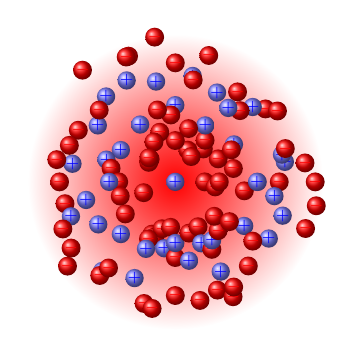
\begin{tikzpicture}[scale=0.75,
		ions/.style={
				circle, ball color=blue!50, font=\tiny, inner sep=0, blue
			},
		electrons/.style={
				circle, ball color=red, font=\tiny, inner sep=0, red
			},
	]
	\path[inner color=red, outer color=white] (0,0) circle(2.5);
	\node[ions] at (0,0) {$+$};
	\pgfmathsetseed{2}
	\foreach \i in {0,10,...,360}
		{
			\node[electrons] at (\i:0.4+1*rnd) {$-$};
			\node[ions] at (\i:1+1*rnd) {$+$};

			\node[electrons] at (\i:1.5+1*rnd) {$-$};
		}
	%		\fill[ball color=red!50]  (45:1.5) coordinate (E2) circle (0.1);
\end{tikzpicture}
			\end{figure}
		\end{column}
		\begin{column}[t]{0.65\linewidth}
			\begin{overprint}
				\onslide<1>
				\begin{block}{}\justifying\small
					За розподілом
					Больцмана концентрації електронів $n_e$:
					\begin{equation*}
						n_e = n\exp{\left( \frac{e\phi}{T}\right) }.
					\end{equation*}

					Далеко від заряду ($r \to \infty$) потенціал поля іона заряду $\phi = 0$, а концентрації іонів та електронів зрівнюються $n_e = n_i  = n$.
				\end{block}
				\onslide<2>
				\begin{block}{}\justifying\small
					Об'ємна густина заряду:
					\begin{equation*}
						\rho = en_i - en_e = en\left[1 - \exp{\left( \frac{e\phi}{T}\right) }\right].
					\end{equation*}
					Для малих значень потенціалу $|e\phi/T \ll 1|$:
					\begin{equation*}
						\rho \approx -\frac{e^2n}{T}\phi
					\end{equation*}
				\end{block}
				\onslide<3>
				\begin{block}{}\justifying\small
					Розподіл потенціалу визначається рівнянням Пуассона $\nabla^2\phi = -4\pi\rho$:
					\begin{equation*}
						\nabla^2\phi = \frac{4\pi e^2n}{T}\phi\ \text{або}\  \nabla^2\phi = \frac{\phi}{r_D^2}
					\end{equation*}
					де
					\begin{equation*}
						\tcbhighmath{\rD .}
					\end{equation*}
				\end{block}
				\onslide<4>
				\begin{block}{}\justifying\small
					Розв'язок рівняння дає:
					\begin{equation*}
						\phi = \frac{e}{r}\exp{\left( -\frac{r}{r_D}\right) }.
					\end{equation*}
					На відстанях порядку $r_D$ відбувається сильне екранування внесеного в плазму заряду:
					\begin{equation*}
						\tcbhighmath{\rD.}
					\end{equation*}
					$r_D$ називають радіусом екранування.
				\end{block}
				\onslide<5>
				\begin{block}{}
					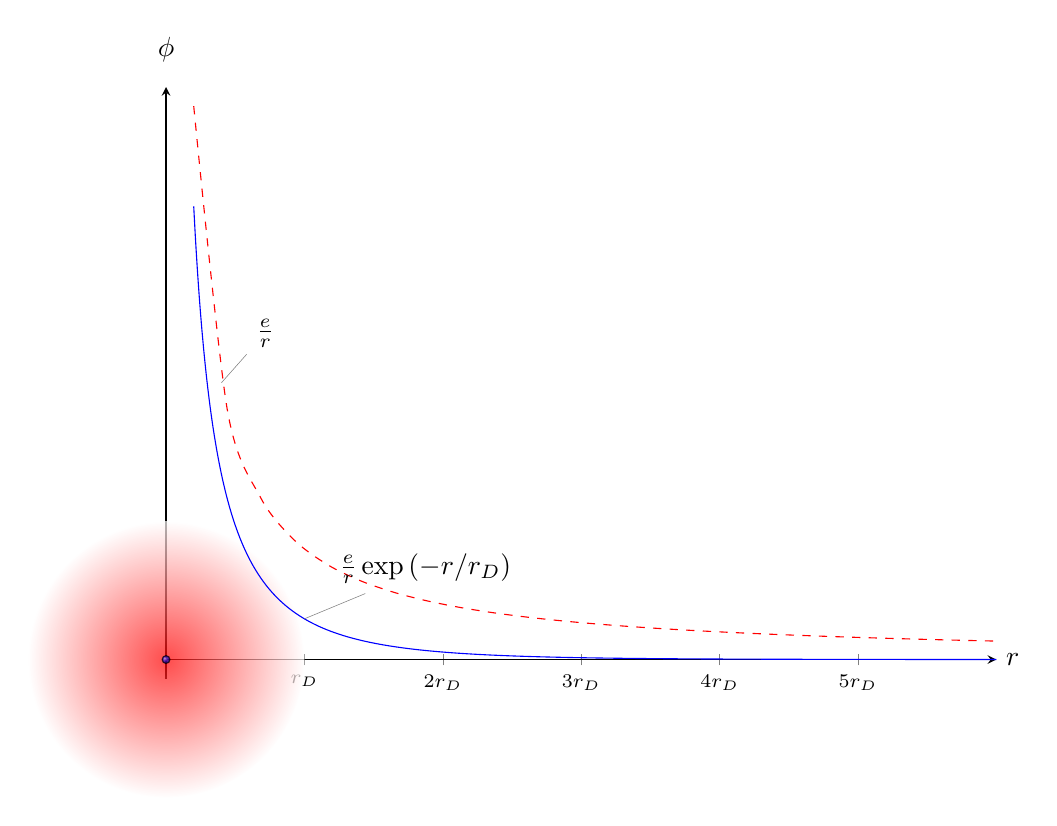
\begin{tikzpicture}
	\begin{axis}[%
            clip=false,
            axis equal,
            xmin=0,
			xlabel=$r$,
			ylabel=$\phi$,
			axis lines=middle,
			every axis x label/.style={at={(current axis.right of origin)},anchor=west},
			every axis y label/.style={at={(current axis.north west)},above=2mm},
			xtick={0.5,1,...,2.5},
            xticklabel={%
                \pgfmathparse{int(\ticknum+1)}
                \ifnum\pgfmathresult>1
                    $\pgfmathresult r_D$
                \else
                    $r_D$
                \fi
            },
            xticklabel style={font=\scriptsize},
			ytick=\empty,
			width=\linewidth,
			height=0.75\linewidth%
		]


        \def\xa{0.2}
        \def\xb{0.5}
        \def\D{0.5}
        \def\q{0.2}

        \begin{scope}[opacity=0.7]
            \path[inner color=red, outer color=white] (axis cs:0,0) circle(\D);
            \draw[ball color=blue] (axis cs:0,0) circle (0.05 cm);
        \end{scope}

		\addplot[red, dashed, domain=0.1:3, smooth, variable=r] {
            % -----------
            \q/r
            % -----------
        };
		\addplot[blue, domain=0.1:3, smooth, variable=r, samples=500] {
            % -----------
            \q/r*exp(-r/\D)
            % -----------
        };

		\node[coordinate,pin={[pin edge={anchor=west}]45:{$\frac{e}{r}\exp{\left(-r/r_D\right)}$} } ] at (axis cs:\xb, {\q/\xb*exp(-\xb/\D)}) {};
		\node[coordinate, pin={[pin edge={anchor=west}]45:{$\frac{e}{r}$} }]
		at (axis cs:\xa, {\q/\xa}) {};

	\end{axis}
\end{tikzpicture}
				\end{block}
			\end{overprint}
		\end{column}
	\end{columns}

	%---------------------------------------------------------
\end{frame}
% ===========================================================================

%% --------------------------------------------------------
\section{Ідеальна та неідеальна плазма}
%% --------------------------------------------------------

% ============================== Слайд ## ===================================
\begin{frame}{Ідеальна та неідеальна плазма}{}
	\framesubtitle<1>{Ідеальна плазма}
	\framesubtitle<2>{Неідеальна плазма}
	\begin{block}{}
		Число частинок в дебаївській сфері:
		\begin{equation*}
			N_D = \frac43\pi r_D^3 n,\ \text{або}\ N \sim \left( \frac{r_D}{d}\right)^3,
		\end{equation*}
		де $d \approx n^{-1/3}$ --- середня відстань між частинками плазми.
	\end{block}
	\begin{overprint}
		\onslide<1>
		\begin{block}{Випадок $N_D \gg 1$ ($r_D \gg d$).}\justifying\scriptsize
			У дебаївській сфері перебуває багато частинок. Оскільки екранування на відстанях, менших за $r_D$, відносно невелике, то домінують колективні ефекти, зумовлені кулонівськими силами, що діють на відстані.
			\begin{equation*}
				\rD \gg n^{-1/3} \Rightarrow \frac{e^2}{d} \ll T.
			\end{equation*}
			Потенціальна енергія \alert{парної} взаємодії частинок мала порівняно з їхньою кінетичною енергією. У цьому разі плазма подібна до \alert{ідеального} газу.
		\end{block}
		%		\onslide<2>
		%		\begin{block}{Випадок $N_D \gg 1$ ($r_D \gg d$).}\justifying\small
		%			З іншого боку
		%			\begin{equation*}
		%				\frac{e^2}{d} \ll T
		%			\end{equation*}
		%			Сенс цієї умови в тому, що потенціальна енергія \alert{парної} взаємодії частинок мала порівняно з їхньою кінетичною енергією. У цьому разі плазма подібна до ідеального газу.
		%
		%			\medskip
		%
		%
		%			Таку плазму називають також \alert{ідеальною}.
		%		\end{block}
		\onslide<2>
		\begin{block}{Випадок $N_D \lesssim 1$ ($r_D \gtrsim d$).}\justifying\scriptsize
			\begin{equation*}
				\rD \lesssim n^{-1/3} \Rightarrow \frac{e^2}{d} \gtrsim T.
			\end{equation*}
			Потенціальна енергія \alert{парної} взаємодії частинок більша або порівняна з їхньою кінетичною енергією. Дебаївське екранування має місце
			тільки в тому випадку, коли в зарядженій хмарі перебуває  досить багато частинок. Однак, за даної умови дебаївське екранування не можна
			вважати статистично правильним поняттям.

			\medskip

			Таку плазму називають \alert{неідеальною}.
			%            А тому поняття <<плазми>> втрачає сенс.
		\end{block}

		%        \begin{alertblock}{}\justifying\centering
		%            Що таке неідеальна плазма?
		%        \end{alertblock}
	\end{overprint}
\end{frame}
% ===========================================================================

% ============================== Слайд ## ===================================
\begin{frame}{Рівняння стану плазми}{}
	\begin{overprint}
		\onslide<1>
		\begin{block}{Енергія плазми}
			\begin{equation*}
				W = \frac32 N_i T_i + \frac32 N_e T_e + \underbrace{ W_{ie} + W_{ii} + W_{ee}}_{%
					\underset{\text{\tiny для квазінейтрального середовища}}{W_\text{кор} \neq 0}%
				}.
			\end{equation*}

		\end{block}
		\onslide<2>
		\begin{block}{Енергія плазми}
			\begin{equation*}
				W = \frac32 N_i T_i + \frac32 N_e T_e + W_\text{кор} = 3nVT\left(1 - \frac{1}{9N_D}\right).
			\end{equation*}
		\end{block}
		\onslide<3>
		\begin{block}{Енергія плазми}
			\begin{equation*}
				W = W_\text{кін} + W_\text{кор}, \quad
				W_\text{кор} = -\frac{e^2}{2r_D}nV.
			\end{equation*}
		\end{block}
	\end{overprint}
	\begin{overprint}
		\onslide<1>
		\begin{block}{Кореляційна енергія}\justifying
			\begin{equation*}
				W_\text{кор} = \frac12\sum_s e_s \delta\phi_s,
			\end{equation*}
			де $\delta\phi_s$ --- потенціал зарядів у точці знаходження розглядуваного за вирахуванням ого власного потенціалу:
			\begin{equation*}
				\delta\phi_s = \left[\frac{e_s}{r}e^{-\frac{r}{r_D}} - \frac{e_s}{r}\right]_{r \to 0} = -\frac{e_s}{r_D} \Rightarrow
				\tcbhighmath{W_\text{кор} = -\frac{e^2}{2r_D}(N_i + N_e).}
			\end{equation*}
		\end{block}
		\onslide<2>
		\begin{block}{Відношення енергій}
			\begin{equation*}
				\gamma = \frac{|W_\text{кор}|}{W_T} = \frac{1}{9 N_D}
			\end{equation*}
			Якщо $\gamma \ll 1$ плазма \alert{ідеальна}, якщо $\gamma \gtrsim 1$ --- плазма \alert{неідеальна}.
		\end{block}

		\begin{exampleblock}{}
			До якого виду належить плазма в центрі Сонця? У центрі зірки <<білий карлик>>?
		\end{exampleblock}
		\onslide<3>
		\begin{alertblock}{}\justifying\scriptsize
			Кореляційна енергія кулонівської взаємодії (на одну частинку) $ W_\text{кор} = -\frac{e^2}{2r_D} $ не співпадає енергією парної взаємодії$ W_\text{пар} = \frac{e^2}{d} \approx - e^2n^{-1/3} $. Відношення енергій:
			\begin{equation*}
				\frac{W_\text{кор}}{W_\text{пар}} = \frac1{N_D^{1/3}}.
			\end{equation*}
			В ідеальній плазмі ($N_D \gg 1$)
			\begin{equation*}
				W_\text{кор} \ll W_\text{пар}.
			\end{equation*}
		\end{alertblock}
		\begin{block}{}\justifying\scriptsize
			Частинки сильно взаємодіють \alert{всередині дебаївської сфери} за допомогою кулонівської взаємодії, що спричиняє колективні ефекти. Однак така взаємодія на енергію плазми впливає не суттєво.
		\end{block}
	\end{overprint}
\end{frame}
% ===========================================================================

\begin{frame}{Види плазми}{Таблиця}
	\begin{equation*}
		r_D\ \text{[см]} = 743\sqrt{\frac{T}{n}}, \quad N_D = 1.7\cdot10^9\sqrt{\frac{T^3}{n}},\quad [T] = \text{еВ},\quad [n] = \text{см}^{-3}.
	\end{equation*}
	\begin{center}
		\pgfplotstabletypeset[
    font=\small,
    col sep=comma,
    header=false,
    columns={0,1,2,3,4},
    columns/0/.style={string type, column type=l},
    columns/1/.style={
        sci,
        retain unit mantissa=false,
        column type=l,
    },
    columns/2/.style={
        sci,
        column type=l
    },
    create on use/3/.style={
                create col/expr={
                7.43e2*sqrt(\thisrowno{2}/\thisrowno{1})
            },
        },
    columns/3/.style={
            sci,
            column type=l,
            precision=0,
        },
    create on use/4/.style={
            create col/expr={
                1.7e9*sqrt(\thisrowno{2}^3/\thisrowno{1})
            },
        },
    columns/4/.style={
            sci,
            sci zerofill,
            column type=l,
            precision=0,
        },
    every head row/.style={%
        output empty row,
        before row={%
            \toprule
            Тип розряду & $n$, см\textsuperscript{-3} & T, еВ & $r_D$, см  & $N_D$ \\
        },
        after row=\midrule,
    },
    every last row/.style={%
        after row=\bottomrule},
]{tikz/data.txt}
	\end{center}
\end{frame}

% ============================== Слайд ## ===================================
\begin{frame}{Види плазми}{Графік}
	\begin{center}
		
\begin{tikzpicture}[pltype/.style={
				font=\tiny\itshape,
				text width=3cm,
				align=center,
				gray
			},
		wraped/.style={
				text width=2cm,
				align=center,
			},
		sz/.style={
				font=\scriptsize,
				fill=white,
				inner sep=0,
				gray!50, opacity=0.75,text opacity=1, sloped
			},
	]
	\begin{axis}[
			ymode=log,
			xmode=log,
			xlabel={$n$, cm$^{-3}$},
			ylabel={$T$, eV},
			xmin=1e-5,
			xmax=1e30,
			ymin=1e-4,
			ymax=1e8,
			% xtick distance={1e3},
			% ytick distance={1e1},
			width=\linewidth,
			height=0.75\linewidth,
			axis background/.style={fill=white},
			label style={font=\scriptsize},
			ticklabel style={font=\scriptsize},
		]


		\def\C{743^2}
		\def\Cn{6.95e-7}
		\only<1>{
			\foreach[count=\c from -2] \n in {-8,-6,...,6} {
					\edef\temp{\noexpand
						\addplot[red!50, domain=1e-5:1e40,
							add node at y={1e\c}{[sz]{$r_D = 10^{\n}$ cm}}
						] {1/\C*(1e\n)^2*x};
					}


					\temp
				}

			\foreach[count=\c from 0] \n in {0,2,...,14} {
					\edef\temp{\noexpand%
						\addplot[blue!20, domain=1e-5:1e40,
							add node at y={10^(2 + \c * 0.6 )}{[sz]{$N_D = 10^{\n}$}}
						] {(\Cn*(1e\n)^(2/3)*x^(1/3))};
					}

					\temp
				}
		}

		\only<2>{
			\addplot[domain=1e-5:1e30, red, name path=Ef,
				add node at y={1e1}{[red, fill=white, sloped]{$T = E_F$}},
			] {3e-16 * x^(2/3)};

			\draw[red] (axis cs:1e-5, 5e5) --node[fill=white] {$T = m_ec^2$} (axis cs:1e30, 5e5);

			\draw[red] (axis cs:1e-5, 5e5) --node[fill=white] {$T = m_ec^2$} (axis cs:1e30, 5e5);

			\addplot[blue, domain=1e-5:1e28, name path=Wcorr,
				add node at y={1e-1}{[fill=white, sloped, red]{$T = W_\text{кор}$}}
			] {(\Cn*(1)^(2/3)*x^(1/3))};

			\draw[red, dashed, name path=KvId] (axis cs:1e28, 1e-4) -- (axis cs:1e28, 1e3);



			\node[pltype] at (axis cs: 1e15, 1e7) {Релятивістська\\ плазма};

			\node[pltype] at (axis cs: 1e3, 1e3) {Класична\\ ідеальна плазма};

			\node[pltype] at (axis cs: 1e14, 1e-3) {Класична\\ неідеальна плазма};

			\node[pltype] at (axis cs: 1e24, 1e-3) {Квантова\\ неідеальна плазма};

			\node[pltype, rotate=90] at (axis cs: 1e29, 1e-1) {Квантова ідеальна плазма};
		}


        \addplot[
        scatter,
        nodes near coords,
        nodes near coords style={font=\scriptsize},
        coordinate style/.condition={\coordindex==0}{text width=2cm, align=center},
        coordinate style/.condition={\coordindex==6}{anchor=south east},
        blue, only marks,
        point meta=explicit symbolic
        ] table [header=false,meta index=0,x index = 1, y index = 2,col sep=comma] {tikz/data.txt};


	\end{axis}
\end{tikzpicture}
	\end{center}
\end{frame}
% ===========================================================================

%% --------------------------------------------------------
\section{Плазмові коливання}
%% --------------------------------------------------------

% ============================== Слайд ## ===================================
\begin{frame}{Плазмові коливання та плазмова частота}{Теплові флуктуації густини плазми}
	\begin{columns}
		\begin{column}{0.3\linewidth}
			\begin{overprint}
				\onslide<1>
				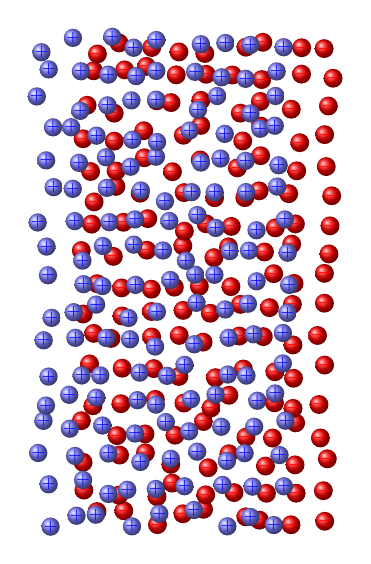
\begin{tikzpicture}[scale=0.75,
		ions/.style={
				circle, ball color=blue!50, font=\tiny, inner sep=0, blue
			},
		electrons/.style={
				circle, ball color=red, font=\tiny, inner sep=0, red
			},
	]

	%        \draw[xshift=0.5cm, fill=gray!50] (0,0) rectangle ++(4,8);
	%        \draw[dashed] (0,0) rectangle ++(4,8);

	\foreach \x in {0,0.5,...,4} {
			\foreach \y in {0,0.5,...,8} {
					\node[ions] at (\x+0.3*rnd,\y+0.3*rnd) {$+$};
					\node[electrons] at ({\x+0.75+0.3*rnd},\y+0.3*rnd) {$-$};
				}
		}
\end{tikzpicture}
				\onslide<2-3>
				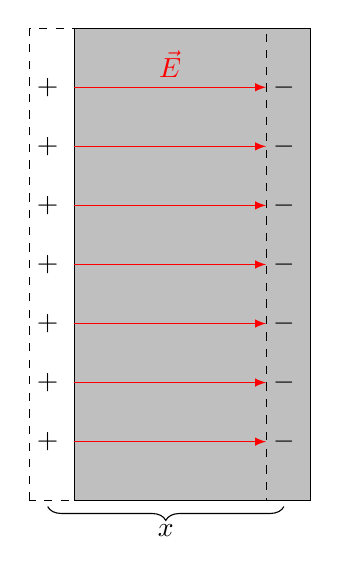
\begin{tikzpicture}[scale=0.75,
		ions/.style={
				circle, ball color=blue!50, font=\tiny, inner sep=0, blue
			},
		electrons/.style={
				circle, ball color=red, font=\tiny, inner sep=0, red
			},
	]

	\draw[xshift=0.75cm, fill=gray!50] (0,0) rectangle ++(4,8);
	\draw[dashed] (0,0) rectangle ++(4,8);

	\foreach \y in {1,...,7} {
			\node at (0.3, \y) {$+$};
			\node at (4.3, \y) {$-$};
			\draw[-latex, red] (0.75, \y) -- (4, \y) \ifnum\y=7 node[above, pos=0.5] {$\vec{E}$} \fi ;
		}

	\draw[decorate,decoration={brace,amplitude=5pt,mirror,raise=0ex}] (0.3,-0.1)  -- (4.3,-0.1) node[midway, yshift=-2ex] {$x$};

\end{tikzpicture}
			\end{overprint}

		\end{column}
		\quad
		\begin{column}{0.7\linewidth}
			\begin{overprint}
				\onslide<1>
				\begin{block}{}\justifying\small
					У розрідженій плазмі відбуваються теплові коливання густини електронної підсистеми. Іони можна вважати нерухомими, оскільки електричне поле спричиняє незрівнянно менший зсув іонів через їхню більшу масу.
				\end{block}
				\begin{center}
					%                    \href{https://i.gifer.com/1yn5.gif}{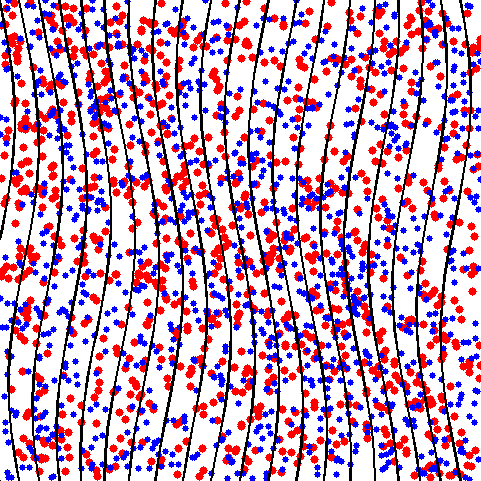
\includegraphics[width=4cm]{plasma_ocillations}}
                    \button{\href{https://youtu.be/-Cz_VnBN7Fg}{Відео}}
                    %					\href{https://youtu.be/-Cz_VnBN7Fg}{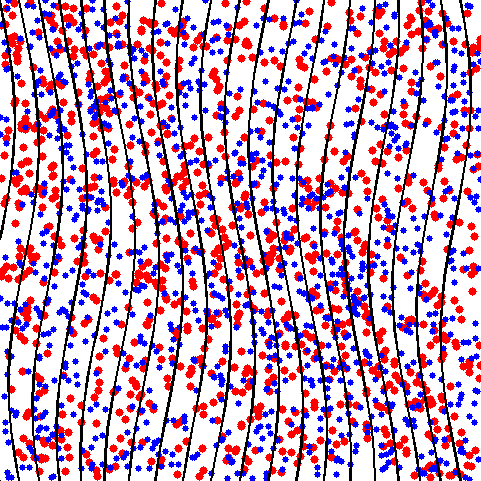
\includegraphics[width=4cm]{plasma_ocillations}}
				\end{center}
				\onslide<2>
				\begin{block}{}\justifying\small
					Виділимо плоский шар електронів. Якщо шар електронів змістився праворуч уздовж осі $x$ перпендикулярно своїй площині на відстань $ x $ від свого початкового положення (коли густина електронів була однорідна, то зліва від шару виникне надлишок позитивного заряду з величиною $\sigma enx$ на одиницю площі шару, тому що під час свого руху шар <<оголює>> іонний остов позаду. Навпаки, праворуч створюється надлишковий негативний заряд $ - \sigma$. У результаті утворюється подоба плоского конденсатора, заряджені обкладки якого формують електричне поле:
					\begin{equation*}
						E = 4\pi\sigma = 4\pi en x
					\end{equation*}
				\end{block}
				\onslide<3>
				\begin{block}{}\justifying\small
					Поле гальмує електрони в шарі, прагнучи повернути їх у вихідне положення, прирівнюючи прискорення електрона в шарі (помножене на масу $m_e$) до сили, що повертає $ -eE$, отримаємо рівняння руху електрона:
					\begin{equation*}
						m_e \ddot{x} = - 4\pi e^2 n x.
					\end{equation*}
					Це рівняння описує коливальний рух із частотою:
					\begin{equation*}
						\tcbhighmath{\omegap.}
					\end{equation*}
					Ця величина називається \alert{плазмовою} (або \alert{ленгмюрівською частотою}).
				\end{block}
			\end{overprint}
		\end{column}
	\end{columns}
\end{frame}
% ===========================================================================


% ============================== Слайд ## ===================================
\begin{frame}{Плазмові коливання та плазмова частота}{Виведення загальним способом}
	\renewcommand{\baselinestretch}{0.85}
	\begin{block}{}\justifying\tiny
		Закон збереження заряду
		\begin{equation}\label{eq:charge_conservation}
			\frac{\partial \rho}{\partial t}  = - \operatorname{div}\vec{j}.
		\end{equation}
		де $\vec{j}$ --- густина струму. Припустимо, що струм переноситься тільки електронами. Тоді

		\begin{equation}\label{eq:current}
			\vec{j}  = - ne\vec{v},
		\end{equation}

		де $\vec{v}$ --- швидкість електронів, що переносять струм ("струмова швидкість"). Рівняння
		руху електрона

		\begin{equation}\label{eq:motion_law}
			m\frac{d\vec{v}}{dt} = -e\vec{E}.
		\end{equation}

		Підставивши вираз \eqref{eq:current} у рівняння \eqref{eq:charge_conservation}, продиференціювавши останнє за часом і підставивши потім рівняння \eqref{eq:motion_law}, отримаємо

		\begin{equation}\label{eq:motion_law2}
			\frac{\partial^2 \rho}{\partial t^2}  = - \frac{ne^2}{m}\operatorname{div}\vec{E}.
		\end{equation}

		При цьому, маючи на увазі лінійні коливання і не роблячи різниці між частковою і повною похідними часу, відкинемо всі квадратичні члени, а $n$ винесемо за знаки диференціалів. За рівнянням Максвелла

		\begin{equation}
			\operatorname{div}\vec{E} = 4\pi \rho.
		\end{equation}

		Підставивши цей вираз у рівняння \eqref{eq:motion_law2}, отримаємо

		\begin{equation}
			\frac{\partial^2 \rho}{\partial t^2}  = - \frac{4\pi ne^2}{m}\rho.
		\end{equation}

		Тепер уже не обкладки уявного конденсатора, а густина об'ємного заряду в плазмі коливається з тією ж круговою частотою:

		\begin{equation*}
			\omegap .
		\end{equation*}
	\end{block}
\end{frame}
% ===========================================================================

% ============================== Слайд ## ===================================
\begin{frame}{Амплітуда плазмових коливань}{}
	\begin{block}{}\justifying\small
		Густина енергії електричного поля:
		\begin{equation*}
			w_e = \frac{E^2}{8\pi} = 2\pi e^2n^2x_{\max}^2
		\end{equation*}
		Ця енергія утворюється за рахунок кінетичної енергії $w_T = nT/2$ теплового руху електронів.

		\medskip

		Звідки, прирівнюючи ці дві енергії $w_T = w_e$, отримуємо:
		\begin{equation*}
			x_{\max} = \sqrt{\frac{T}{4\pi e^2n}} = r_D.
		\end{equation*}

		Амплітуду швидкості цих коливань можна оцінити як $v_{\max} = \omega_p r_D$:

		\begin{equation*}
			v_{\max}  = \sqrt{\frac{4\pi ne^2}{m}} \sqrt{\frac{T}{4\pi e^2n}} = \sqrt{\frac{T}{m}} = v_T,
		\end{equation*}
		де $v_T$ --- теплова швидкість електронів.

	\end{block}
\end{frame}
% ===========================================================================

% ============================== Слайд ## ===================================
\begin{frame}{Плазмові коливання в металах}{}
\begin{columns}
	\begin{column}{0.5\linewidth}
        \begin{center}
            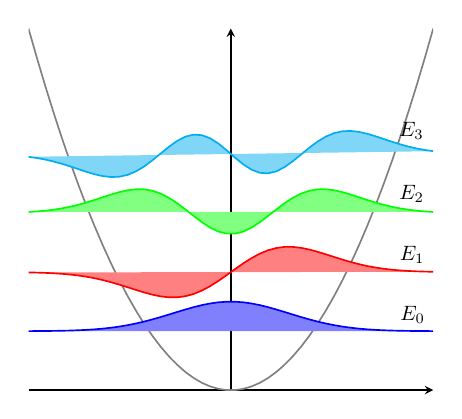
\begin{tikzpicture}[scale=0.75]
    \begin{axis}[domain=-3.5:3.5,
    xtick=\empty,
    ytick=\empty,
    samples=50,
    no markers,
    axis lines=middle,
    y=1cm,
    thick]
    \addplot [gray] {1/2*x^2};
    \addplot[fill=blue!50, draw=blue] {1/(2*sqrt(1*1!))*exp(-x^2/2)+1} node[pos=0.95, above] {$E_0$};
    \addplot[fill=red!50, draw=red] {1/(2*sqrt(2*1!))*2*x*exp(-x^2/2)+2} node[pos=0.95, above] {$E_1$};
    \addplot[fill=green!50, draw=green] {1/(2*sqrt(4*2!))*(4*x^2-2)*exp(-x^2/2)+3} node[pos=0.95, above] {$E_2$};
    \addplot[fill=cyan!50, draw=cyan] {1/(2*sqrt(8*3!))*(8*x^3-12*x)*exp(-x^2/2)+4} node[pos=0.95, above] {$E_3$};
    \end{axis}
\end{tikzpicture}
        \end{center}
	\end{column}
	\begin{column}{0.5\linewidth}
         \begin{block}{}\justifying\scriptsize
            Плазму в металі можна розглядати як квантовий гармонічний осцилятор. Якщо обстрілювати електронами алюмінієву фольгу і дуже точно вимірювати їхню енергію, то можна очікувати, електрони будуть втрачати якраз енергію $\hbar\omega_p$. Уперше це явище спостерігалося експериментально в $1936$~р. Електрони з енергіями від кількох тисяч електронвольт, розсіюючись від тонкої металевої фольги або проходячи крізь неї, втрачали енергію порціями. Ефект залишався незрозумілим до $1953$~р., поки \href{https://doi.org/10.1103/PhysRev.92.609}{Бом і Пайнс}  не показали, що все це можна пояснити квантовим збудженням плазми в металі.
         \end{block}
	\end{column}
\end{columns}



\end{frame}
% ===========================================================================

%% --------------------------------------------------------
\section{Основні формули}
%% --------------------------------------------------------

% ============================== Слайд ## ===================================
\begin{frame}{Основні формули}
	\framesubtitle<1>{Теоретичні формули}
	\framesubtitle<2>{Практичні формули}
	\begin{overprint}
		\onslide<1>
		Дебаївський радіус:
		\begin{equation*}
			\rD
		\end{equation*}

		Ленгмюрівська частота:
		\begin{equation*}
			\omegap .
		\end{equation*}

        Число частинок в дебаївській сфері:
        \begin{equation*}
            N = \frac43\pi r_D^3 n
        \end{equation*}
		\onslide<2>
		Дебаївський радіус:
		\begin{equation*}
			r_D = 743\sqrt{\frac{T}{n}}, \quad [T] = \text{еВ},\ [n] = \text{см}^{-3}.
		\end{equation*}

		Ленгмюрівська частота:
		\begin{equation*}
			\omega_p = 5.64\cdot10^4\sqrt{n},\ [n] = \text{см}^{-3}.
		\end{equation*}

          Число частинок в дебаївській сфері:
          \begin{equation*}
              N = 1.7\cdot 10^{9}\frac{T^3}{n},\ [T] = \text{еВ},\ [n] = \text{см}^{-3}.
          \end{equation*}
	\end{overprint}
\end{frame}
% ===========================================================================


%% --------------------------------------------------------
\section{Задачі}
%% --------------------------------------------------------


% ============================== Слайд ## ===================================

\begin{frame}{Задачі}{}
	\begin{overprint}
		\onslide<1>

		\begin{exampleblock}{\stepcounter{probcnt}\scriptsize Задача \theprobcnt}\justifying\scriptsize
			Показати, що квадрат дебаївського радіуса неізотермічної плазми, в якій температури електронного та іонного компонентів різні ($T_e \neq T_i$) пропорційний приведеній температурі $T^* = \dfrac{T_eT_i}{T_e + T_i}$.
		\end{exampleblock}

		\begin{exampleblock}{\stepcounter{probcnt}\scriptsize Задача \theprobcnt}\justifying\scriptsize
			Обчисліть тиск, який чинить  термоядерна плазма на стінки пастки. Припустіть, що $T_e = T_i = 20$~кеВ, $n_e = 10^{21}$~м\textsuperscript{3}.
		\end{exampleblock}
		\begin{exampleblock}{\stepcounter{probcnt}\scriptsize Задача \theprobcnt}\justifying\scriptsize
			Дейтерієва ізотермічна плазма з концентрацією дейтронів $n = 10^{22}$ м\textsuperscript{-3} має температуру $T = 10^7$~К. Обчислити дебаївський радіус екранування та число іонів усередині сфери Дебая.
			% $r_d \approx 1.5 \cdot 10^{-4}$ см, N_D = 1ю6 \свще 1^4.
		\end{exampleblock}
		\begin{exampleblock}{\stepcounter{probcnt}\scriptsize Задача \theprobcnt}\justifying\scriptsize
			У лазерному термоядерному синтезі серцевина крихітної таблетки з
			суміші дейтерію з тритієм стискається до густини $10^{33}$ м\textsuperscript{-3} за
			температури $50\ 000\ 000$~К. Оцініть для такої плазми число частинок у дебаївській сфері.
		\end{exampleblock}
		\onslide<2>
		\setcounter{probcnt}{5}
		\begin{exampleblock}{\scriptsize Задача \theprobcnt}\justifying\scriptsize
			Плоский конденсатор заповнений плазмою із середньою
			концентрацією електронів та іонів $n_0$ і температурою $T$. Відстань
			між пластинами конденсатора $a$, різниця потенціалів $V$.
			Нехтуючи струмом через плазму і вважаючи $eV \ll kT$, визначити
			просторову залежність потенціалу в плазмі між пластинами
			конденсатора.
			% \phi(x) = V $\frac{\sh x/r_D}{\sh a/r_D}$.
		\end{exampleblock}

		\begin{exampleblock}{\stepcounter{probcnt}\scriptsize Задача \theprobcnt}\justifying\scriptsize
			Сферичний провідник радіусом $a$ занурений у плазму і заряджений до потенціалу $\phi_0$. Електрони мають максвеллівський розподіл за швидкостями і рухаються таким чином, щоб утворити дебаївський шар; іони за час експерименту залишаються нерухомими. Припускаючи, що $e\phi_0 \ll T$, знайдіть, як залежність потенціалу $\phi$ від $r$ та величин $a$, $\phi_0$ і $r_D$.
		\end{exampleblock}

		%       \begin{exampleblock}{\stepcounter{probcnt}\scriptsize Задача \theprobcnt}\justifying\scriptsize
		%           Знайти вирази для вільної енергії Гельмгольца, ентропії та тиску ізотермічної плазми температурою $T$.
		%       \end{exampleblock}

		\begin{exampleblock}{\stepcounter{probcnt}\scriptsize Задача \theprobcnt}\justifying\scriptsize
			Частота видимого світла дорівнює приблизно $6\cdot10^{14}$ c\textsuperscript{-1}. Якою має бути густина електронів, щоб отримати таку саму плазмову
			частоту? Порівняти отримане значення густини з густиною
			електронів у типовому атомі радіуса порядку $10^{-8}$~см.
		\end{exampleblock}

		\onslide<3>
		\begin{exampleblock}{\stepcounter{probcnt}\scriptsize Задача \theprobcnt}\justifying\scriptsize
			При отриманні формули для частоти плазмових коливань вважалося,
			що йони знаходяться в спокої. З'ясувати, як впливає врахування руху йонів на значення плазмової частоти?
		\end{exampleblock}

	\end{overprint}
\end{frame}
% ===========================================================================

\end{document}
